\documentclass[10pt,letterpaper]{article}
\usepackage[margin=0.73in]{geometry}
\usepackage{amsmath,amssymb,booktabs,array,graphicx,float,microtype}
\usepackage[round,authoryear]{natbib}
\usepackage[dvipsnames]{xcolor}
\usepackage[colorlinks=true,linkcolor=MidnightBlue,citecolor=MidnightBlue,urlcolor=MidnightBlue]{hyperref}
\usepackage{fancyhdr}\pagestyle{fancy}\fancyhf{}\lhead{FINC B9339 | Homework 3}\rhead{FX carry}\cfoot{\thepage}
\setlength{\headheight}{14pt}\setlength{\parindent}{0pt}\setlength{\parskip}{5pt}
\setlength{\intextsep}{8pt}\renewcommand{\arraystretch}{1.06}
\newcommand{\rBaseSharpe}{0.62942}
\newcommand{\rBaseArith}{5.93551}
\newcommand{\rBaseGeom}{5.64307}
\newcommand{\rBaseVol}{9.43011}
\newcommand{\rBaseDD}{29.57103}
\newcommand{\rBaseSkew}{-0.46649}
\newcommand{\rBaseKurt}{11.54375}
\newcommand{\rBaseES}{1.50005}
\newcommand{\rBaseWorst}{-5.18244}
\newcommand{\rCondSharpe}{1.19913}
\newcommand{\rCondES}{1.02206}
\newcommand{\rCondDD}{8.40631}
\newcommand{\rCondActive}{74.51412}
\newcommand{\rCondBaseSharpe}{0.57981}
\newcommand{\rCondBaseSkew}{-0.46169}
\newcommand{\rCondSkew}{-0.52428}
\newcommand{\rConstDD}{22.64560}
\newcommand{\rVolMatchDD}{20.40108}
\newcommand{\rActiveES}{1.13870}
\newcommand{\rOffProfits}{349}
\newcommand{\rOffCompound}{-22.58560}
\newcommand{\rLagBase}{0.58096}
\newcommand{\rLagAY}{1.13340}
\newcommand{\rLagSix}{1.16447}
\newcommand{\rLagPrimaryAY}{1.19878}
\newcommand{\rCICondLow}{0.18205}
\newcommand{\rCICondHigh}{1.07016}
\newcommand{\rHistSharpe}{0.95487}
\newcommand{\rHistDD}{14.73348}
\newcommand{\rHistES}{1.10999}
\newcommand{\rHistSkew}{-0.40746}
\newcommand{\rEBaseSharpe}{0.55638}
\newcommand{\rEImpliedSharpe}{1.16706}
\newcommand{\rEImpliedES}{1.02498}
\newcommand{\rEImpliedSkew}{-0.52597}
\newcommand{\rCIDiffLow}{-0.07908}
\newcommand{\rCIDiffHigh}{0.58620}
\newcommand{\rSizeEffect}{0.08028}
\newcommand{\rMethodEffect}{0.03505}
\newcommand{\rTenorEffect}{0.01269}
\newcommand{\rSpreadGeom}{6.11324}
\newcommand{\rSpreadVol}{12.75363}
\newcommand{\rSpotMean}{1.89340}
\newcommand{\rCarryMean}{4.04203}
\newcommand{\rInteractionMean}{0.00008}
\newcommand{\rVixCorr}{-0.48127}
\newcommand{\rAYCorr}{-0.30297}
\newcommand{\rVixCrisis}{-0.69063}
\newcommand{\rLowES}{0.99306}
\newcommand{\rHighES}{2.20394}
\newcommand{\rLowMean}{0.03369}
\newcommand{\rHighMean}{-0.01190}
\newcommand{\rCrisisBase}{-20.10077}
\newcommand{\rCrisisAY}{-6.87929}
\newcommand{\rCrisisHistorical}{-6.05593}
\begin{document}
\begin{center}{\Large\bfseries FX Carry and Volatility Conditioning}\\[5pt]
Columbia Business School | Systematic Investment Strategies\\
Professor Achilles Venetoulias | Fall 2026\end{center}
\section*{Summary of answers (a)--(e)}
\textbf{(a) Twelve portfolios.} Combine 1M/3M interest rates, two/three currencies on each side,
and equal/rank/median-spread allocation. At each daily close, buy the highest-yield currencies
and short the lowest-yield currencies. Long and short initial USD notionals sum to $+1$ and $-1$;
weights determined at $t$ earn the return from $t$ to the next observation. All 12 dated holdings
are shown in Section 2, and complete daily weights accompany the submission.

\textbf{(b) Baseline comparison.} The highest sample Sharpe is the \textbf{3M, three-per-side,
equal-weight} portfolio: \textbf{\rBaseSharpe{}}. Annual arithmetic/geometric returns are
\textbf{\rBaseArith{}\%/\rBaseGeom{}\%}, volatility \textbf{\rBaseVol{}\%}, and maximum drawdown
\textbf{\rBaseDD{}\%}. Skewness is \rBaseSkew{} and excess kurtosis \rBaseKurt{}.
Adding a third currency per side has the largest mean absolute paired Sharpe effect
(\rSizeEffect{} versus \rMethodEffect{} for weighting and \rTenorEffect{} for tenor).

\textbf{(c) Volatility relationship.} Carry correlates negatively with changes in all six
volatility indicators. Pearson correlations are \rAYCorr{} with AY3M changes and \rVixCorr{}
with VIX changes; the latter becomes \rVixCrisis{} in 2008. \textbf{AY3M} is a reasonable
conditioning candidate: next-day ES rises from \rLowES{}\% in its low regime to \rHighES{}\%
in its high regime. AY1wk is essentially tied on that risk contrast and has unusually stale quotes.
The data support Jurek's qualitative stress relationship, not an estimate of his crash premium.

\textbf{(d) Six filters.} The fixed prior-252-observation 75th-percentile rule selects
\textbf{AY3M} by sample Sharpe: \rCondSharpe{}, versus \rCondBaseSharpe{} unfiltered on the same
2,727 dates. It is active \rCondActive{}\% of the time, with drawdown \rCondDD{}\% and daily
ES \rCondES{}\%. A constant portfolio with equal average exposure has drawdown \rConstDD{}\%:
reduced exposure alone does not explain the outcome. However, one additional decision lag
changes the highest-Sharpe filter to AY6M. The winner is timing-sensitive.

\textbf{(e) Historical volatility.} A 21-day AUD/JPY realized-volatility filter has Sharpe
\rHistSharpe{}, versus \rEImpliedSharpe{} for AY3M and \rEBaseSharpe{} unfiltered on the common
2,707 dates. Drawdown is \rHistDD{}\%, versus \rCondDD{}\% for AY3M. AY3M wins on point estimates,
but a paired block-bootstrap interval for its Sharpe advantage over the historical filter is
[\rCIDiffLow{}, \rCIDiffHigh{}], which includes zero. Historical filtering loses less during 2008.

\textbf{Scope.} This is an in-sample, zero-cost comparison using 1999--2010 data, not an
out-of-sample ranking. Filtering reduces exposure; it does not purchase option insurance.
\newpage
\section{Data, returns and evaluation conventions}
The CSV contains 2,981 weekday observations from January 1, 1999 through June 4, 2010,
producing 2,980 holding returns. The universe is EUR, JPY, GBP, CAD, AUD, NZD, CHF, NOK and SEK;
USD supplies the matching funding rate. All spot and 20 yield series are complete. Five FX
implied-volatility series are complete, while VIX has 108 missing entries (at most four consecutive).
All supplied rows, including holidays, are retained. AY1wk has a 289-observation constant run
in 2002--2003, a data-quality limitation retained without unsupported corrections.

Yields and FX implied volatilities are annualized percentages; VIX is in percentage points.
The analysis uses the CSV consistently. The accompanying XLSX contains the same spot levels
but some higher-precision yields and volatilities; the two sources are not mixed.

\subsection{Quotation normalization and exact USD excess return}
Let $X_{i,t}$ be USD per unit of foreign currency. EUR, GBP, AUD and NZD already have this
convention; invert JPY, CAD, CHF, NOK and SEK. Arithmetic spot returns are
$s_{i,t+1}=X_{i,t+1}/X_{i,t}-1$. Returns are calculated directly from normalized spot levels at full available precision.
The supplied foreign ROR columns are rounded to four decimal places, with half-unit rounding
tolerance 0.00005, and are not used in the portfolio calculations.
For example, a fall in JPY/USD means yen appreciation and a positive USD-per-yen return.

Quoted yields $p_{i,t}$ are converted to decimals, $y_{i,t}=p_{i,t}/100$, and treated as
continuously compounded daily financing proxies. For actual calendar days divided by 365,
$\Delta_t=(\mathrm{date}_{t+1}-\mathrm{date}_t)/365$,
\begin{align}
x_{i,t+1}&=e^{y_{i,t}\Delta_t}\frac{X_{i,t+1}}{X_{i,t}}-e^{y_{USD,t}\Delta_t},\\
R_{t+1}&=\sum_i w_{i,t}x_{i,t+1}.
\end{align}
A USD of foreign deposit grows at the foreign yield and is converted back at the next spot;
subtract the matched USD funding growth. Signed weights represent lending or foreign borrowing.
The common USD term cancels because $\sum_iw_{i,t}=0$, but foreign interest does not cancel.
The exact decomposition is
\[
x_{i,t+1}=s_{i,t+1}+\left(e^{y_{i,t}\Delta_t}-e^{y_{USD,t}\Delta_t}\right)
+\left(e^{y_{i,t}\Delta_t}-1\right)s_{i,t+1}.
\]
Thus additive spot plus yield differential is only approximate. Baseline annual arithmetic
contributions are \rSpotMean{}\% spot, \rCarryMean{}\% carry and \rInteractionMean{}\% interaction.
One-/three-month rates proxy daily borrowing/lending; no term-deposit mark-to-market is modeled.
The original rate compounding basis is not identified by the dataset. ACT/365 gives three days'
accrual over weekends. Negative yields are allowed.

\subsection{Performance definitions}
Using $N$ daily arithmetic excess returns, sample standard deviation $s_R$ (divisor $N-1$),
and 252 observations per year,
\[
\mu_A=252\bar R,\quad \sigma_A=\sqrt{252}s_R,\quad SR=\sqrt{252}\bar R/s_R,\quad
G_A=\left[\prod_{t=1}^{N}(1+R_t)\right]^{252/N}-1.
\]
Funding is already included: do not subtract USD interest again for Sharpe. Skewness and Fisher
excess kurtosis use bias-corrected sample estimates. With a linear empirical quantile $q_{.05}$,
$VaR_{.05}=-q_{.05}$ and $ES_{.05}=-\operatorname{mean}\{R_t:R_t\le q_{.05}\}$.
For $W_0=1$, $W_t=\prod_{u\le t}(1+R_u)$, drawdown is
$D_t=W_t/\max(1,W_1,\ldots,W_t)-1$ and $MDD=-\min_tD_t$.
Loss VaR/ES/MDD are positive; worst daily returns are signed. Wealth is a compounded
excess-return index, not a cash balance including collateral interest.
\newpage
\section{Daily allocations: answer (a)}
At close $t$, rank the nine foreign yields for each tenor, select the top $k$ and bottom $k$,
$k\in\{2,3\}$, and hold until the next observation. This gives $2\times2\times3=12$ constructions.
Normalize each side separately: long $+1$, short $-1$, gross initial USD notional $2$ per unit
of collateral. Net initial notional zero does not imply zero exposure to all market risk factors.

\textbf{Equal allocation:} each selected currency has absolute weight $1/k$.
\textbf{Rank allocation:} within each side, weights are proportional to $k,k-1,\ldots,1$;
the highest-yield long and lowest-yield short receive the largest absolute weights.
\textbf{Median-spread allocation:} let $m_t$ be the median of all nine foreign yields. Then
\[
w_{i,t}=\frac{y_{i,t}-m_t}{\sum_{j\in L_t}(y_{j,t}-m_t)}\ (i\in L_t),\qquad
w_{i,t}=-\frac{m_t-y_{i,t}}{\sum_{j\in S_t}(m_t-y_{j,t})}\ (i\in S_t).
\]
This adapts Jurek's spread idea to nine foreign currencies; it does not reproduce his
ten-currency center or monthly rebalancing. Alphabetical order breaks tied yields.
Selected spreads must be nonnegative; a zero selected spread receives zero weight,
and an all-zero side falls back to equal allocation. Neither zero-spread event occurs here.
Yield ties occur on 17 dates for 1M and 91 for 3M, so a deterministic tie rule matters.

The table gives decisions at close September 12, 2008, earning the return ending September 15.
It explicitly states all 12 allocations; rounded weights need not sum exactly to one on paper.
Full-precision weights for every decision/holding date and two additional snapshots are supplied.
\begin{table}[H]\centering\small\caption{All 12 dated portfolios; E=equal, R=rank, S=median-spread}\begin{tabular}{l >{\raggedright\arraybackslash}p{5.8cm} >{\raggedright\arraybackslash}p{5.8cm}}\toprule Tenor/$k$/method & Long weights & Short weights\\\midrule
1M/2/E & AUD +0.50000; NZD +0.50000 & JPY -0.50000; CHF -0.50000\\[4pt]
1M/2/R & AUD +0.33333; NZD +0.66667 & JPY -0.66667; CHF -0.33333\\[4pt]
1M/2/S & AUD +0.43139; NZD +0.56861 & JPY -0.61058; CHF -0.38942\\[4pt]
1M/3/E & AUD +0.33333; NZD +0.33333; NOK +0.33333 & JPY -0.33333; CAD -0.33333; CHF -0.33333\\[4pt]
1M/3/R & AUD +0.33333; NZD +0.50000; NOK +0.16667 & JPY -0.50000; CAD -0.16667; CHF -0.33333\\[4pt]
1M/3/S & AUD +0.35299; NZD +0.46527; NOK +0.18174 & JPY -0.48168; CAD -0.21111; CHF -0.30721\\[4pt]
3M/2/E & AUD +0.50000; NZD +0.50000 & JPY -0.50000; CHF -0.50000\\[4pt]
3M/2/R & AUD +0.33333; NZD +0.66667 & JPY -0.66667; CHF -0.33333\\[4pt]
3M/2/S & AUD +0.44155; NZD +0.55845 & JPY -0.63113; CHF -0.36887\\[4pt]
3M/3/E & AUD +0.33333; NZD +0.33333; NOK +0.33333 & JPY -0.33333; CAD -0.33333; CHF -0.33333\\[4pt]
3M/3/R & AUD +0.33333; NZD +0.50000; NOK +0.16667 & JPY -0.50000; CAD -0.16667; CHF -0.33333\\[4pt]
3M/3/S & AUD +0.35135; NZD +0.44437; NOK +0.20429 & JPY -0.49977; CAD -0.20812; CHF -0.29210\\[4pt]
\bottomrule\end{tabular}\end{table}

These are dynamic positions. The 1M equal two-per-side portfolio initially buys GBP/NOK and
shorts JPY/CHF; the displayed snapshot instead buys AUD/NZD. The selected baseline is always
short JPY and almost always short CHF, while AUD/NZD are frequent longs. This motivates
AUD/JPY volatility but does not make it a complete risk measure for the changing basket.

\textbf{Timing assumption.} Holdings and yields dated $t$ are used only for $R_{t+1}$.
Same-date observations are assumed available at a common daily fixing; timestamps are not
provided. Portfolio returns begin after the observations used to set holdings, conditional on
this common-fixing assumption. The timing sensitivity analysis below delays both selection
and risk exposure by one additional observation.
\newpage
\section{Baseline performance: answer (b)}
Select the highest sample Sharpe, then higher geometric return, lower ES and lower drawdown
if needed; an alphabetical label resolves an exact remaining tie. This same rule selects
filtered portfolios. The required allocation grid and fixed filter settings are evaluated without an additional
parameter search. The winning labels are nevertheless selected in sample. All baselines use the same 2,980 dates.
\begin{table}[H]\centering\small\caption{All 12 baselines: January 4, 1999--June 4, 2010}
\begin{tabular}{lrrrrr}\toprule
Strategy & Arith.\% & Geom.\% & Vol.\% & Sharpe & $W_N$\\\midrule
1M\_2\_equal & 6.54030 & 5.95866 & 12.24641 & 0.53406 & 1.98266\\
1M\_2\_rank & 6.29816 & 5.61585 & 12.89331 & 0.48848 & 1.90812\\
1M\_2\_spread & 6.74996 & 6.11324 & 12.75363 & 0.52926 & 2.01714\\
1M\_3\_equal & 5.85791 & 5.56736 & 9.36863 & 0.62527 & 1.89779\\
1M\_3\_rank & 6.07803 & 5.64037 & 10.85403 & 0.55998 & 1.91337\\
1M\_3\_spread & 6.24082 & 5.80901 & 10.88294 & 0.57345 & 1.94980\\
3M\_2\_equal & 6.30371 & 5.66370 & 12.58489 & 0.50090 & 1.91837\\
3M\_2\_rank & 6.44590 & 5.70234 & 13.39277 & 0.48130 & 1.92668\\
3M\_2\_spread & 6.65922 & 5.96480 & 13.13094 & 0.50714 & 1.98402\\
3M\_3\_equal & 5.93551 & 5.64307 & 9.43011 & 0.62942 & 1.91395\\
3M\_3\_rank & 6.19070 & 5.72643 & 11.13738 & 0.55585 & 1.93188\\
3M\_3\_spread & 6.37574 & 5.93640 & 11.01433 & 0.57886 & 1.97774\\
\bottomrule\end{tabular}\end{table}
\begin{table}[H]\centering\small\caption{Baseline risk: daily 5\% VaR/ES and full-path drawdown}
\begin{tabular}{lrrrrrr}\toprule
Strategy & Skew & Ex.kurt. & MDD\% & Worst\% & VaR\% & ES\%\\\midrule
1M\_2\_equal & -0.54779 & 7.30342 & 38.03704 & -5.44509 & 1.21017 & 2.01383\\
1M\_2\_rank & -0.60639 & 8.90520 & 42.92287 & -6.85405 & 1.21530 & 2.10865\\
1M\_2\_spread & -0.58356 & 7.99469 & 40.78760 & -6.02413 & 1.21966 & 2.09484\\
1M\_3\_equal & -0.41379 & 11.10755 & 29.68471 & -5.18133 & 0.89481 & 1.47931\\
1M\_3\_rank & -0.56238 & 10.31977 & 36.45722 & -6.01769 & 1.04650 & 1.76110\\
1M\_3\_spread & -0.60141 & 9.45705 & 35.90266 & -5.51539 & 1.03014 & 1.77411\\
3M\_2\_equal & -0.53310 & 10.74438 & 40.33509 & -6.52349 & 1.19491 & 2.05277\\
3M\_2\_rank & -0.57307 & 10.50329 & 44.04632 & -6.85538 & 1.26206 & 2.18213\\
3M\_2\_spread & -0.61323 & 10.32265 & 43.00755 & -6.44166 & 1.22104 & 2.14205\\
3M\_3\_equal & -0.46649 & 11.54375 & 29.57103 & -5.18244 & 0.89766 & 1.50005\\
3M\_3\_rank & -0.53780 & 11.57892 & 37.01960 & -6.01891 & 1.06993 & 1.80400\\
3M\_3\_spread & -0.63670 & 10.76940 & 36.41298 & -5.74553 & 1.02972 & 1.78949\\
\bottomrule\end{tabular}\end{table}

The selected baseline has Sharpe \rBaseSharpe{}, geometric return \rBaseGeom{}\%, daily ES
\rBaseES{}\% and drawdown \rBaseDD{}\%. It does not dominate every metric: the
1M/two-per-side/spread portfolio earns geometric return \rSpreadGeom{}\%, but at volatility
\rSpreadVol{}\%, versus \rBaseVol{}\% for the selected portfolio.

All 12 return distributions are negatively skewed and heavy-tailed. The selected portfolio's
worst day is \rBaseWorst{}\%; a Gaussian description would omit economically important crash
exposure. Appendix~\ref{app:figures} presents the full histograms and 2008 portfolio paths.
\newpage
\subsection{Paired design comparisons and the crisis}
Each comparison holds the other two design choices fixed. Averaging absolute Sharpe changes
gives the following descriptive ranking; weighting has three pairwise contrasts per cell.
\begin{table}[H]\centering\small\caption{Average absolute paired design effects}
\begin{tabular}{lrrr}\toprule
Dimension & Pairs & $|\Delta SR|$ & $|\Delta G|$ (pp)\\\midrule
k & 6 & 0.08028 & 0.13219\\
method & 12 & 0.03505 & 0.22225\\
tenor & 6 & 0.01269 & 0.13651\\
\bottomrule\end{tabular}\end{table}

The number of currencies per side is the largest Sharpe influence. Three per side improves
Sharpe in all six matched comparisons, consistent with lower concentration. Equal allocation
beats rank/spread in all four tenor/size cells. The tenor comparison is mixed: 1M wins four of
six Sharpe pairs; the two leading equal three-per-side portfolios are very close. For geometric
return instead of Sharpe, allocation has the largest paired effect. ``Most influential'' is
therefore metric-dependent rather than a universal structural conclusion.
\begin{figure}[H]\centering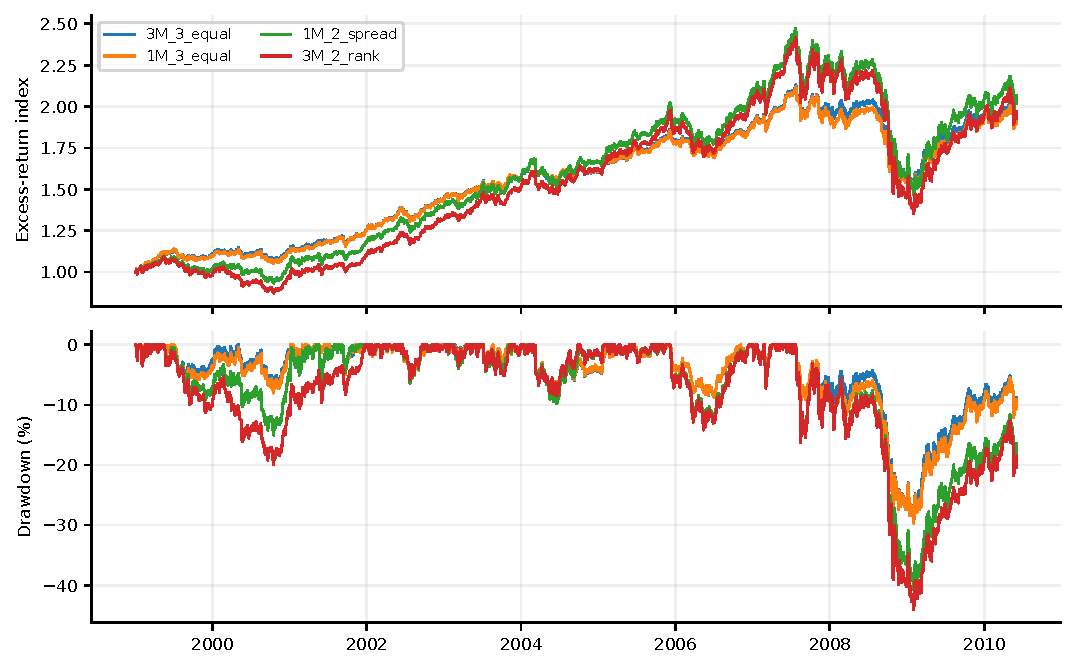
\includegraphics[width=\linewidth,height=3.6in,keepaspectratio]{../results/figures/review_baseline_paths.pdf}\caption{Four representative constructions illustrate diversification, concentration and return trade-offs. Appendix~\ref{app:figures} shows complete paths for all twelve portfolios.}\end{figure}

All portfolios lose in 2008; calendar compounded losses range from about 18.91\% to 33.48\%.
The chosen baseline returns \rCrisisBase{}\% during that year. Its crisis loss confirms that
interest accrual does not eliminate currency crash risk. Figure~\ref{appfig:baseline_2008}
compares all twelve constructions during the crisis.

Calendar-period return is $W_N-1$, distinct from annualized geometric return. There are 262
supplied weekday observations in 2008, while the stipulated annualization remains 252.
\newpage
\section{Volatility and carry: answer (c)}
\citet{jurek2014} documents negatively skewed carry returns and equity-downside exposure,
then studies option-based crash hedges. His hedged strategies retain positive mean excess
returns, and his estimated crash-risk share is at most about one third of carry compensation.
Those option-price results are not implied by a successful volatility filter. The Barclays framework \citep{barclays2011} motivates
simple systematic risk-premium portfolios and recognizes losses when underlying risks materialize.
These readings motivate a stress hypothesis; they do not establish that this sample must agree.

\subsection{Contemporaneous comovement}
Compute $\operatorname{Corr}(R_t,V_t-V_{t-1})$ using actual raw observations, not imputed
volatility changes. The same 2,769 dates are used for all six indicators (244 in 2008).
Pearson measures linear association; Spearman uses ranks and is less dominated by the largest
changes. Neither is, by itself, a forecast test.
\begin{table}[H]\centering\small\caption{Same-day carry returns and volatility changes}
\begin{tabular}{lrrr}\toprule
Indicator & Pearson & Spearman & Pearson 2008\\\midrule
AY1wk & -0.30874 & -0.15114 & -0.47188\\
AY3M & -0.30297 & -0.13838 & -0.47096\\
AY6M & -0.28826 & -0.13577 & -0.48447\\
JPY3M & -0.38447 & -0.20927 & -0.57639\\
AUD3M & -0.30962 & -0.16437 & -0.39038\\
VIX & -0.48127 & -0.27772 & -0.69063\\
\bottomrule\end{tabular}\end{table}

All signs are negative. VIX has the strongest contemporaneous association, \rVixCorr{} overall
and \rVixCrisis{} in 2008. JPY3M is the strongest FX measure contemporaneously. This supports
common stress exposure, but not causality or a priced crash premium. VIX is broad 30-day equity
volatility, not Jurek's equity put-writing/downside factor.

\subsection{Decision-date levels and subsequent losses}
At close $t$, compare $V_t$ with terciles of its preceding 252 as-of values; then group
$R_{t+1}$. Low is at/below the lower tercile, high is strictly above the upper tercile.
These relative regimes use no full-sample thresholds and need not have equal counts.
All six comparisons use the same 2,727 dates, December 23, 1999--June 4, 2010.
\begin{table}[H]\centering\small\caption{Next-day conditional means and 5\% ES, all in daily \%}
\begin{tabular}{lrrrrrr}\toprule
Indicator & Mean low & Mean mid & Mean high & ES low & ES mid & ES high\\\midrule
AY1wk & 0.03349 & 0.05360 & -0.01862 & 0.99458 & 1.37106 & 2.20523\\
AY3M & 0.03369 & 0.04425 & -0.01190 & 0.99306 & 1.40378 & 2.20394\\
AY6M & 0.02900 & 0.05194 & -0.00895 & 1.06122 & 1.28922 & 2.23369\\
JPY3M & 0.03065 & 0.03551 & -0.00611 & 1.11104 & 1.30762 & 2.22829\\
AUD3M & 0.03781 & 0.05582 & -0.01460 & 0.99107 & 1.30732 & 2.07361\\
VIX & 0.02680 & 0.04141 & 0.00217 & 1.12559 & 1.15288 & 2.13657\\
\bottomrule\end{tabular}\end{table}

AY3M's low/high next-day means are \rLowMean{}\%/\rHighMean{}\%, while ES rises from
\rLowES{}\% to \rHighES{}\%. Its high-minus-low ES contrast is the largest, but less than one thousandth of a percentage point above AY1wk's: this is effectively a tie, not reliable statistical
separation. AY3M is a defensible candidate because AUD/JPY links frequent investment/funding
positions and its three-month tenor avoids especially persistent AY1wk quotes. The ES ranking
is exploratory and does not establish out-of-sample forecasting performance.
\newpage
\subsection{Economic interpretation and Jurek comparison}
AY1wk, AY3M and AY6M measure the same AUD/JPY cross over different horizons. A longer tenor
may smooth near-term noise but may react differently to a sudden shock. JPY3M relates to the
persistent yen funding short; AUD3M relates to a frequent investment currency. VIX captures
broader equity stress. None spans all changing NZD, NOK, CHF, CAD and other exposures.

High observed volatility can mark persistent stress and larger subsequent losses, while rising
volatility can simply accompany a loss already realized. The distinction explains why VIX's
strong same-day correlation need not produce the best next-day filter. Figure~\ref{appfig:predictive_regime_distributions}
compares subsequent return distributions across the observed regimes.
\begin{figure}[H]\centering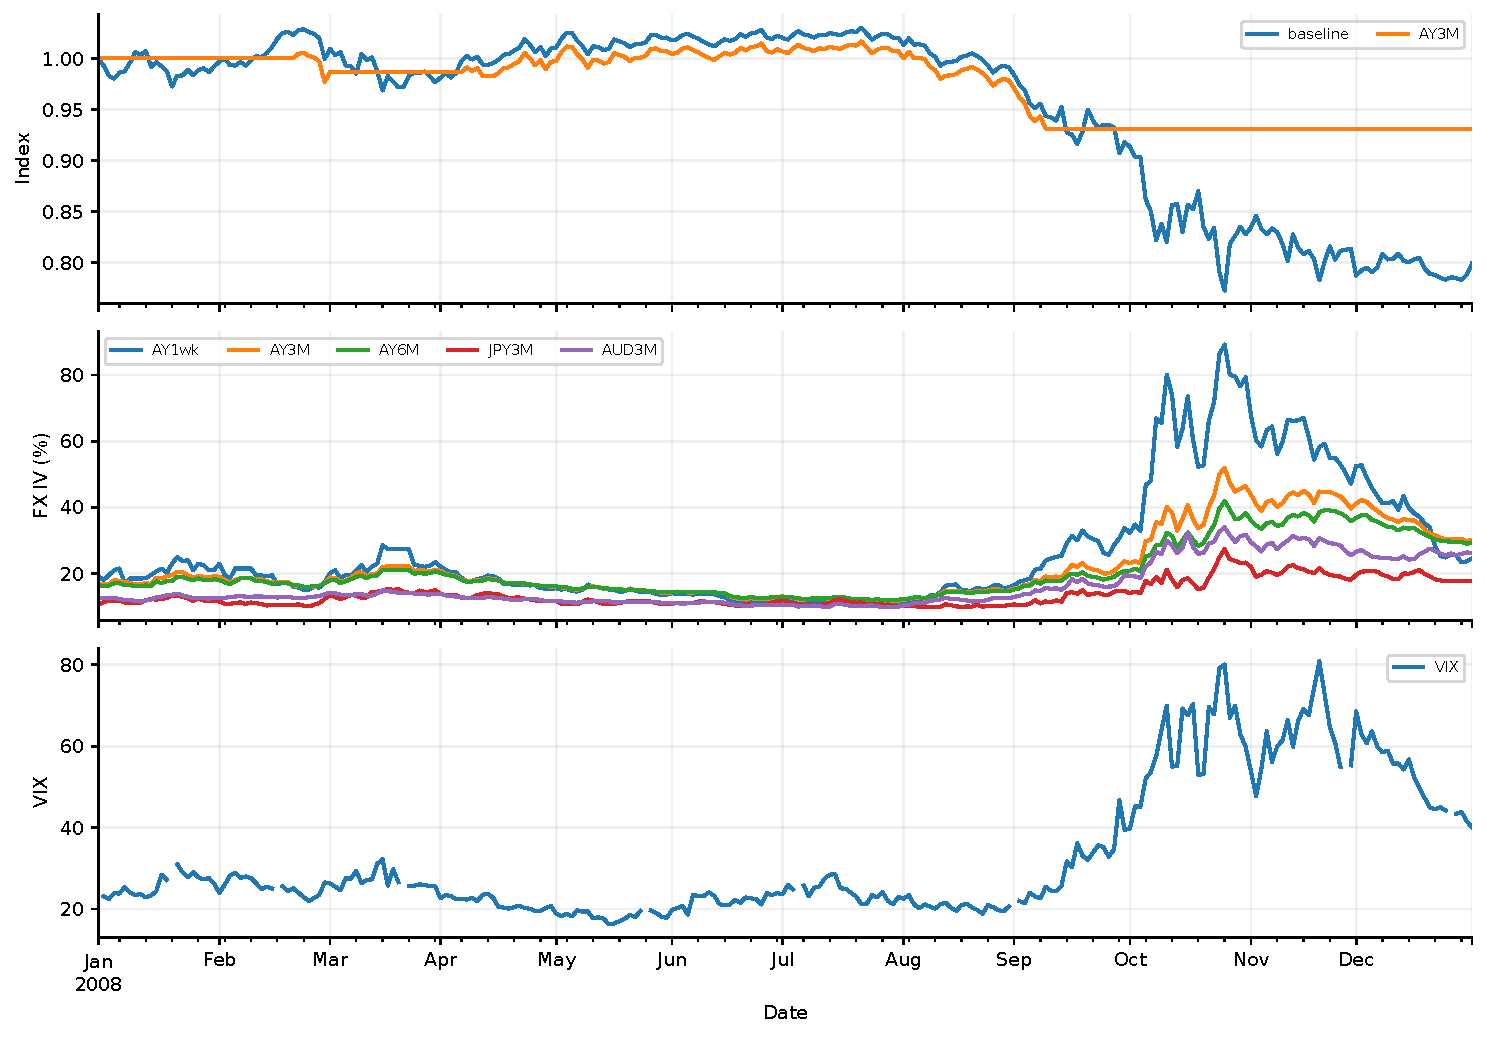
\includegraphics[width=\linewidth,height=3.9in,keepaspectratio]{../results/figures/stress_2008.pdf}\caption{2008: unfiltered and AY3M-filtered wealth, the five FX implied volatilities, and VIX. The filtered strategy remains exposed until the risk signal switches off.}\end{figure}

\textbf{Do the data confirm Jurek?} They support the qualitative stress relationship:
negative baseline skewness (\rBaseSkew{}), excess kurtosis (\rBaseKurt{}), a large 2008 loss,
and negative contemporaneous FX/equity-volatility correlations. They do not reproduce his
option-hedging or risk-premium result. Jurek uses monthly rebalancing, a different sample
(1990--2012), and actual options; this study uses daily positions and no option payoffs.
His Section 5.4.1 compares risk-neutral and realized moments. Our filtered-return difference
cannot identify either a variance risk premium or the fraction of carry compensation due to crashes.

\section{Fixed volatility filters: answer (d)}
For each indicator, define
\[
q_t=Q_{.75}(V_{t-252},\ldots,V_{t-1}),\qquad z_t=\mathbf{1}\{V_t\le q_t\},
\qquad R^{(V)}_{t+1}=z_tR_{t+1}.
\]
Lookback, percentile and exposure levels (one/zero) are fixed, not optimized. Risk-off earns
zero excess return. Percentiles are linear-interpolated and exclude $V_t$.
Missing volatility is forward-filled only after its first observation; the window counts
252 prior as-of values, including carried VIX values. No spot/yield imputation or partial
warm-up is used. All six filters and benchmark share the same 2,727-date evaluation window.
\newpage
\subsection{All six conditioned return distributions}
\begin{table}[H]\centering\small\caption{Conditioned strategies: common-period central performance}
\begin{tabular}{lrrrrr}\toprule
Strategy & Arith.\% & Geom.\% & Vol.\% & Sharpe & Active\%\\\midrule
baseline & 5.59118 & 5.25860 & 9.64310 & 0.57981 & 100.00000\\
AY1wk & 6.69079 & 6.67735 & 6.72167 & 0.99541 & 74.77081\\
AY3M & 7.69799 & 7.77834 & 6.41966 & 1.19913 & 74.51412\\
AY6M & 6.98934 & 7.01498 & 6.45536 & 1.08272 & 75.54089\\
JPY3M & 6.84691 & 6.83682 & 6.81948 & 1.00402 & 78.47451\\
AUD3M & 7.09391 & 7.13959 & 6.27138 & 1.13116 & 68.24349\\
VIX & 5.84090 & 5.78496 & 6.57641 & 0.88816 & 74.33077\\
\bottomrule\end{tabular}\end{table}
\begin{table}[H]\centering\small\caption{Conditioned strategies: shape and downside risk}
\begin{tabular}{lrrrrr}\toprule
Strategy & Skew & Ex.kurt. & MDD\% & Worst\% & ES\%\\\midrule
baseline & -0.46169 & 11.46287 & 29.57103 & -5.18244 & 1.54309\\
AY1wk & -0.49904 & 5.09784 & 9.08370 & -2.48685 & 1.07094\\
AY3M & -0.52428 & 5.08578 & 8.40631 & -2.48685 & 1.02206\\
AY6M & -0.58396 & 5.26657 & 10.41034 & -2.53898 & 1.03416\\
JPY3M & -0.60733 & 5.51732 & 13.80880 & -2.58245 & 1.09489\\
AUD3M & -0.38444 & 6.01371 & 9.08259 & -2.48685 & 0.99939\\
VIX & -0.53289 & 5.43982 & 10.19340 & -2.48685 & 1.06197\\
\bottomrule\end{tabular}\end{table}

AY3M wins under the same Sharpe criterion used for the baseline. It agrees with the exploratory
part (c) candidate, but agreement was not guaranteed: part (c) compares tercile risk contrasts,
whereas the trading rule switches at the 75th percentile. AUD3M has smaller daily ES and volatility
than AY3M, so the selected winner is not best on every risk measure.

Filtering improves loss magnitudes but does not eliminate asymmetry. AY3M skewness
(\rCondSkew{}) is more negative than unfiltered skewness (\rCondBaseSkew{}) on this sample.
Zero-return risk-off days alter unconditional quantiles and create a point mass at zero;
standardized moments need not improve when drawdowns fall.

The winning filter still skips \rOffProfits{} profitable days. Compounding all skipped-day
carry returns gives \rOffCompound{}\%; that realized negative total explains why switching off
helped here, not why it must help in the future. No additional leverage restores the lost
average exposure. During 2008, AY3M returns \rCrisisAY{}\%, versus \rCrisisBase{}\% unfiltered;
it protects imperfectly and does not win every subperiod.

Comparing all six indicators is necessary because contemporaneous association, predictive risk
separation, and the payoff of a particular switch-off threshold are different questions.
Common, untuned parameters make the comparison interpretable. Selecting the best of six after
observing results still creates selection bias.

\textbf{Filtering versus insurance.} This rule can remain invested before a sudden shock,
react after losses, and re-enter when historical thresholds adapt to elevated absolute risk.
It buys no put and guarantees no loss floor. It is therefore not Jurek's crash-neutral overlay.
\newpage
\subsection{Exposure controls, timing and statistical uncertainty}
A constant reference with exposure $p=\operatorname{mean}(z_t)$ has returns $pR_t$.
Positive constant scaling leaves Sharpe unchanged. Its exposure level is measured ex post,
so it serves as a descriptive benchmark rather than an implementable trading rule. A second reference
scales the baseline to the filter's realized volatility. Both controls use the same dates.
\begin{table}[H]\centering\small\caption{Downside protection beyond uniform exposure reduction}
\begin{tabular}{lrrrr}\toprule
Indicator & Filter MDD\% & Equal-$p$ MDD\% & Equal-vol MDD\% & Active-day ES\%\\\midrule
AY1wk & 9.08370 & 22.71747 & 21.29115 & 1.19461\\
AY3M & 8.40631 & 22.64560 & 20.40108 & 1.13870\\
AY6M & 10.41034 & 22.93281 & 20.50662 & 1.14954\\
JPY3M & 13.80880 & 23.74960 & 21.57804 & 1.20292\\
AUD3M & 9.08259 & 20.87674 & 19.96176 & 1.14847\\
VIX & 10.19340 & 22.59425 & 20.86383 & 1.18553\\
\bottomrule\end{tabular}\end{table}

For AY3M, uniform average-exposure scaling gives drawdown \rConstDD{}\%, and matching realized
volatility gives \rVolMatchDD{}\%, both above the filter's \rCondDD{}\%. ES restricted to active
days is \rActiveES{}\%. Thus the primary sample contains useful timing beyond merely taking
less exposure, although an ex-post control does not establish a causal or future timing premium.

The dataset lacks common-fixing timestamps. The timing sensitivity analysis delays \emph{both}
currency selection and the risk-exposure decision by one further observation, retaining funding
rates known at the holding period's start. Primary and delayed rules below share 2,726 dates
from December 24, 1999. The additional lag is fixed in advance and is not optimized.
\begin{table}[H]\centering\small\caption{Additional lag on both selection and exposure}
\begin{tabular}{lrr}\toprule
Indicator & Primary Sharpe & Extra-lag Sharpe\\\midrule
AY1wk & 0.99504 & 0.96510\\
AY3M & 1.19878 & 1.13340\\
AY6M & 1.08235 & 1.16447\\
JPY3M & 1.00367 & 1.03333\\
AUD3M & 1.13078 & 1.11182\\
VIX & 0.88776 & 0.77708\\
\bottomrule\end{tabular}\end{table}

AY3M falls from \rLagPrimaryAY{} to \rLagAY{}, while AY6M reaches \rLagSix{} and becomes the
winner. The lagged unfiltered benchmark has Sharpe \rLagBase{}. The broad filtering benefit
persists under the additional lag, but the exact winning indicator changes.
\begin{table}[H]\centering\small\caption{Paired moving-block bootstrap: filter minus baseline Sharpe}
\begin{tabular}{lrrr}\toprule
Indicator & $\Delta SR$ & 95\% lower & 95\% upper\\\midrule
AY1wk & 0.41559 & -0.03695 & 0.84243\\
AY3M & 0.61932 & 0.18205 & 1.07016\\
AY6M & 0.50291 & 0.08140 & 0.97193\\
JPY3M & 0.42421 & -0.01100 & 0.88183\\
AUD3M & 0.55134 & 0.08152 & 0.99838\\
VIX & 0.30835 & -0.15251 & 0.73904\\
\bottomrule\end{tabular}\end{table}

Intervals resample paired realized return vectors in 20-observation blocks, with 2,000 draws
and seed 9339. They are pointwise, conditional on the selected baseline and realized rules;
thresholds and the selection procedure are not re-estimated. AY3M's interval is
[\rCICondLow{}, \rCICondHigh{}], but it is not corrected for choosing among 12 baselines and
six filters. These intervals do not establish out-of-sample significance or superiority.
\newpage
\section{Historical versus implied volatility: answer (e)}
Construct AUD/JPY in yen per AUD using the supplied market quotations:
\[
C_t=(USD/AUD)_t(JPY/USD)_t=AUD_t\,JPY_t,\quad u_t=C_t/C_{t-1}-1,
\quad H_t=\sqrt{252}\operatorname{sd}(u_{t-20},\ldots,u_t).
\]
The 21-return sample standard deviation has divisor 20. $H_t$ includes the close-$t$ return
and can condition only $R_{t+1}$. The cross return is computed directly, not approximated by
subtracting arithmetic USD returns. This proxy represents a frequent carry pair but omits
other currencies and the full covariance of actual holdings.

Apply exactly the same prior-252-value 75th-percentile rule. After the realized-volatility
warm-up, all three strategies share January 20, 2000--June 4, 2010, or 2,707 return dates.
The best FX-implied filter is AY3M; it also happens to win among all six indicators including VIX.
\begin{table}[H]\centering\small\caption{Historical comparison: identical evaluation dates}
\begin{tabular}{lrrrrr}\toprule
Strategy & Arith.\% & Geom.\% & Vol.\% & Sharpe & Active\%\\\midrule
baseline & 5.37905 & 5.03306 & 9.66802 & 0.55638 & 100.00000\\
FX\_AY3M & 7.50142 & 7.56620 & 6.42760 & 1.16706 & 74.32582\\
historical & 6.64775 & 6.61398 & 6.96196 & 0.95487 & 75.76653\\
\bottomrule\end{tabular}\end{table}
\begin{table}[H]\centering\small\caption{Historical comparison: complete distributional risk}
\begin{tabular}{lrrrrrr}\toprule
Strategy & Skew & Ex.kurt. & MDD\% & Worst\% & VaR\% & ES\%\\\midrule
baseline & -0.45909 & 11.41468 & 29.57103 & -5.18244 & 0.94453 & 1.54751\\
FX\_AY3M & -0.52597 & 5.08607 & 8.40631 & -2.48685 & 0.63055 & 1.02498\\
historical & -0.40746 & 5.24815 & 14.73348 & -2.58245 & 0.67807 & 1.10999\\
\bottomrule\end{tabular}\end{table}
\begin{figure}[H]\centering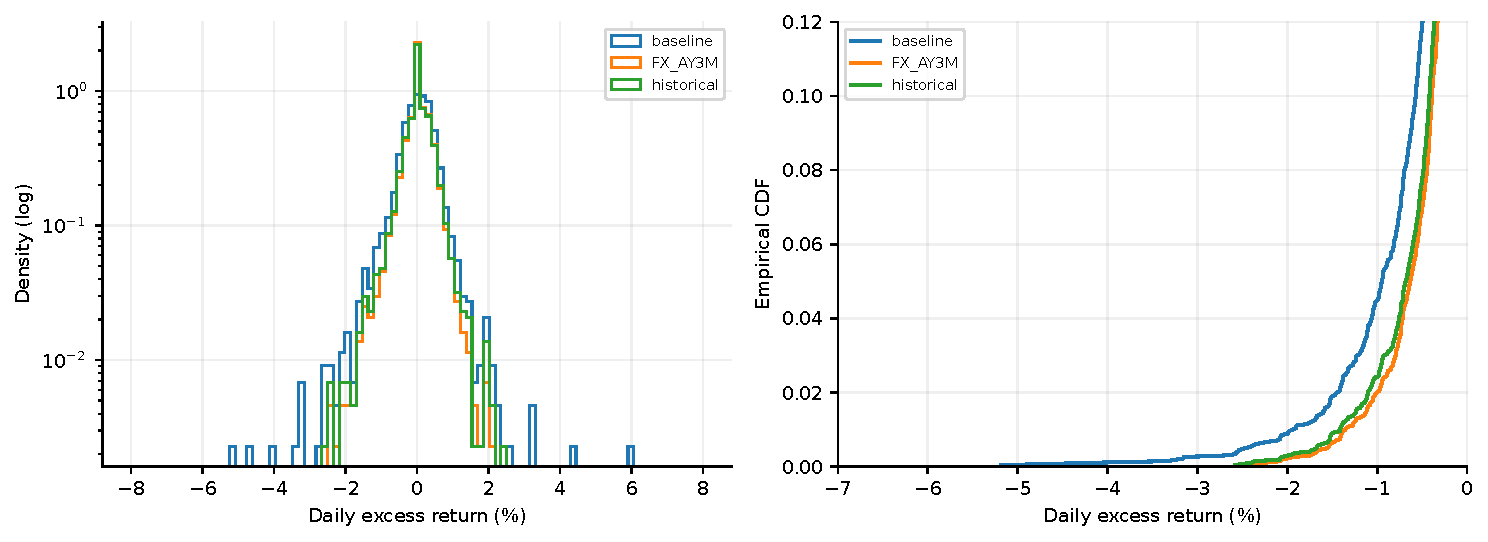
\includegraphics[width=\linewidth,height=2.6in,keepaspectratio]{../results/figures/historical_distributions.pdf}\caption{Unconditional daily distributions, including zero-exposure days, and the lower-tail empirical CDF on the common sample.}\end{figure}

Historical filtering improves risk-adjusted performance relative to unfiltered carry. AY3M's
point estimates are better for Sharpe, drawdown and ES (\rEImpliedES{}\% versus \rHistES{}\%).
Historical skewness (\rHistSkew{}) is less negative than AY3M's (\rEImpliedSkew{}), and its
2008 return (\rCrisisHistorical{}\%) exceeds AY3M's (\rCrisisAY{}\%). The comparison therefore
contains trade-offs, not uniform dominance.
\newpage
\subsection{Information content and limits}
\begin{figure}[H]\centering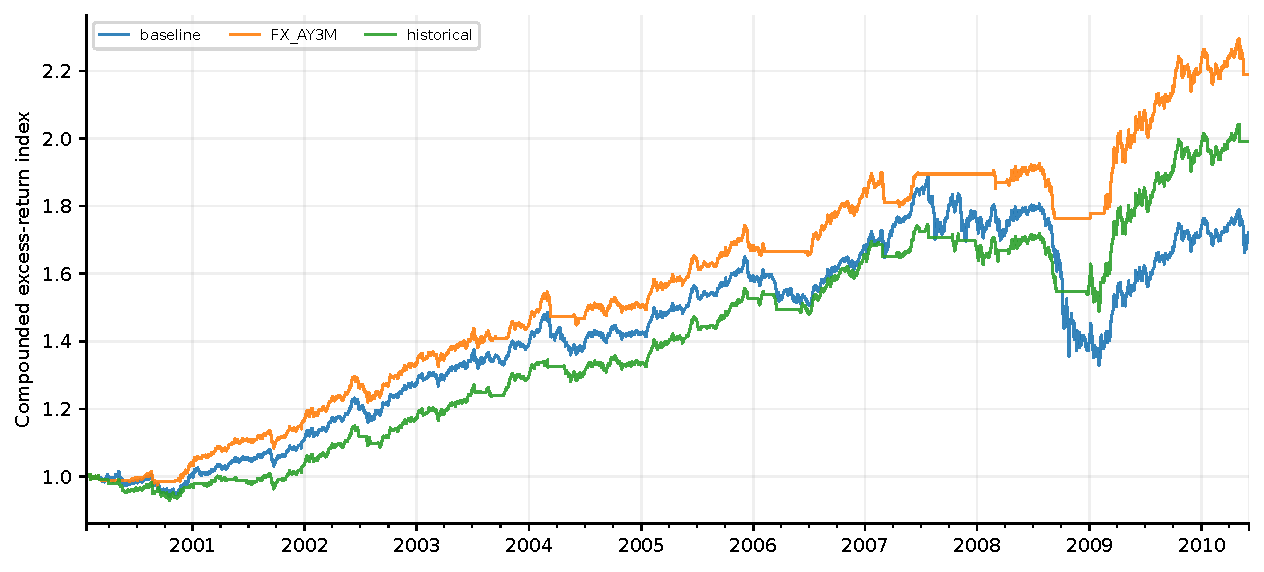
\includegraphics[width=\linewidth,height=2.5in,keepaspectratio]{../results/figures/historical_wealth.pdf}\caption{Compounded excess-return indices for the three strategies on the common historical comparison sample.}\end{figure}

Implied volatility reflects option prices over a future horizon under a risk-neutral measure;
it can contain insurance premia and market frictions rather than a pure physical forecast.
Realized volatility summarizes past physical spot movements. A 21-day measure can react only
after a shock enters its window, but repeated shocks may make it a useful persistent risk signal.
A forward-looking label alone does not guarantee better investment performance.

Here AY3M has the better point-estimate Sharpe, but the paired block-bootstrap interval for
AY3M minus historical Sharpe is [\rCIDiffLow{}, \rCIDiffHigh{}]. It includes zero even before
accounting for model selection. A three-month implied horizon and a 21-day realized window
also differ, so this is not a controlled identification of the value of implied information.
Both filters use relative thresholds and imperfect AUD/JPY risk coverage.

Jurek's implied-versus-realized-moment analysis motivates these distinctions. No option payoff,
option-implied skewness surface, matched variance claim, or equity downside index is available
here; the filtered return difference cannot recover his variance or crash-risk premium.

\section{Conclusion}
The preferred baseline is diversified equal-weight daily carry, but every construction retains
substantial crash exposure. All six volatility filters improve sample Sharpe under the primary
convention; AY3M has the highest point estimate. Exposure-matched controls support a timing
benefit in this sample, while timing sensitivity and the uncertain implied-versus-historical difference
limit claims about a unique winner. These findings support Jurek's qualitative stress evidence
without reproducing his option-hedging conclusions.

The conclusions depend on the assumed availability of spot rates, yields and volatility at a
common daily fixing. Transaction costs are excluded as stipulated by the assignment, and all
strategy selections remain in sample. The results therefore describe historical risk--return
trade-offs rather than a demonstrated out-of-sample investment advantage.
Appendix~\ref{app:figures} provides the complete graphical comparisons.

\bibliographystyle{plainnat}\bibliography{references}

\clearpage
\appendix
\section{Additional graphical evidence}\label{app:figures}
The following figures complete the graphical comparisons for answers (b)--(e).
All twelve baseline constructions and all six volatility filters are shown.
The wealth, distribution and stress figures already in the main text are not repeated.
Return conventions and evaluation samples are the same as in the corresponding tables.
\setcounter{figure}{0}
\renewcommand{\thefigure}{A.\arabic{figure}}
\renewcommand{\theHfigure}{appendix.\arabic{figure}}
\begin{figure}[H]\centering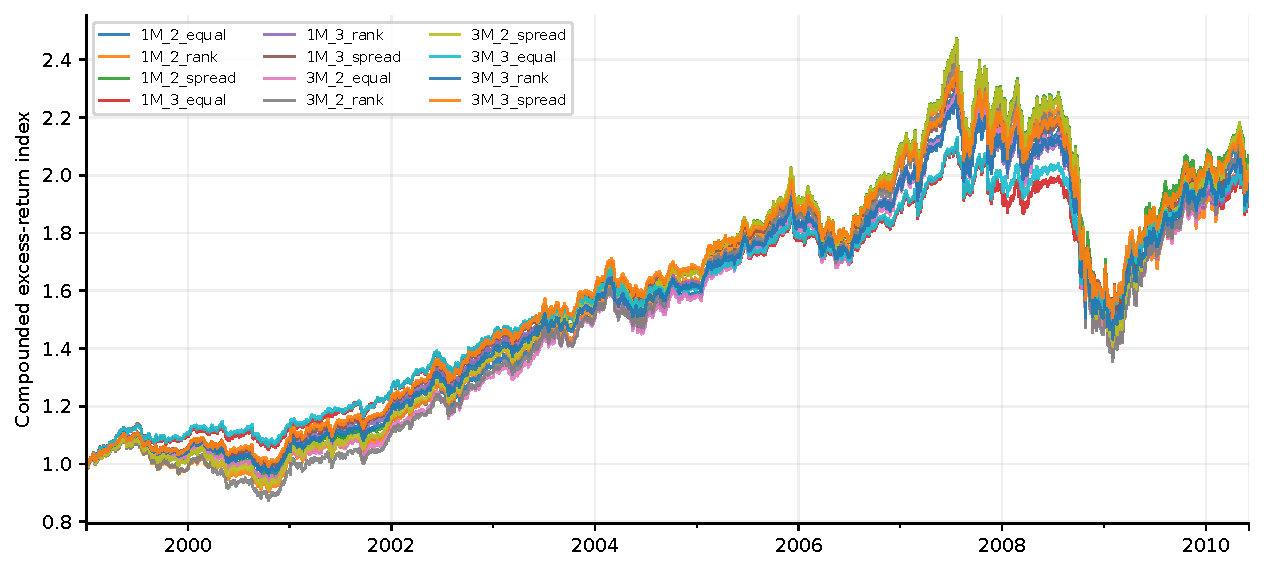
\includegraphics[width=\linewidth,height=6.2in,keepaspectratio]{../results/figures/baseline_wealth.pdf}\caption{\textbf{All twelve baseline wealth paths.} Daily compounded excess-return indices over the full 2,980-return baseline sample. The complete paths complement the representative constructions in the main text.}\label{appfig:baseline_wealth}\end{figure}
\clearpage
\begin{figure}[H]\centering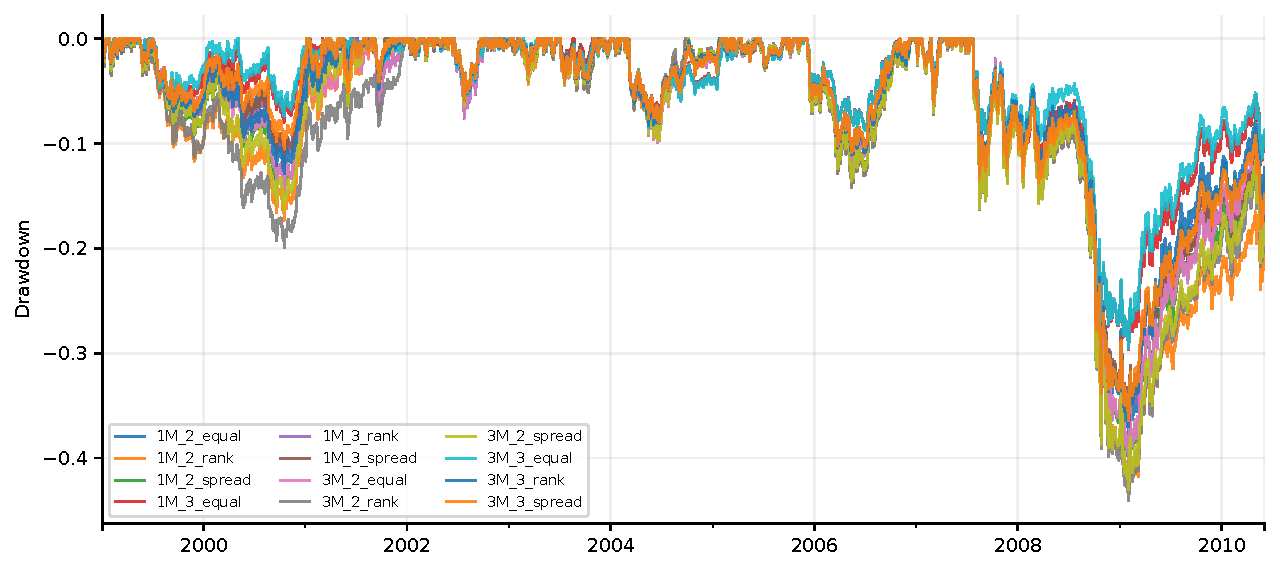
\includegraphics[width=\linewidth,height=6.2in,keepaspectratio]{../results/figures/baseline_drawdowns.pdf}\caption{\textbf{All twelve baseline drawdown paths.} Losses relative to previous wealth peaks, including initial wealth one, over the same baseline sample. Drawdowns here are signed fractions; reported maximum drawdown statistics are positive loss percentages.}\label{appfig:baseline_drawdowns}\end{figure}
\clearpage
\begin{figure}[H]\centering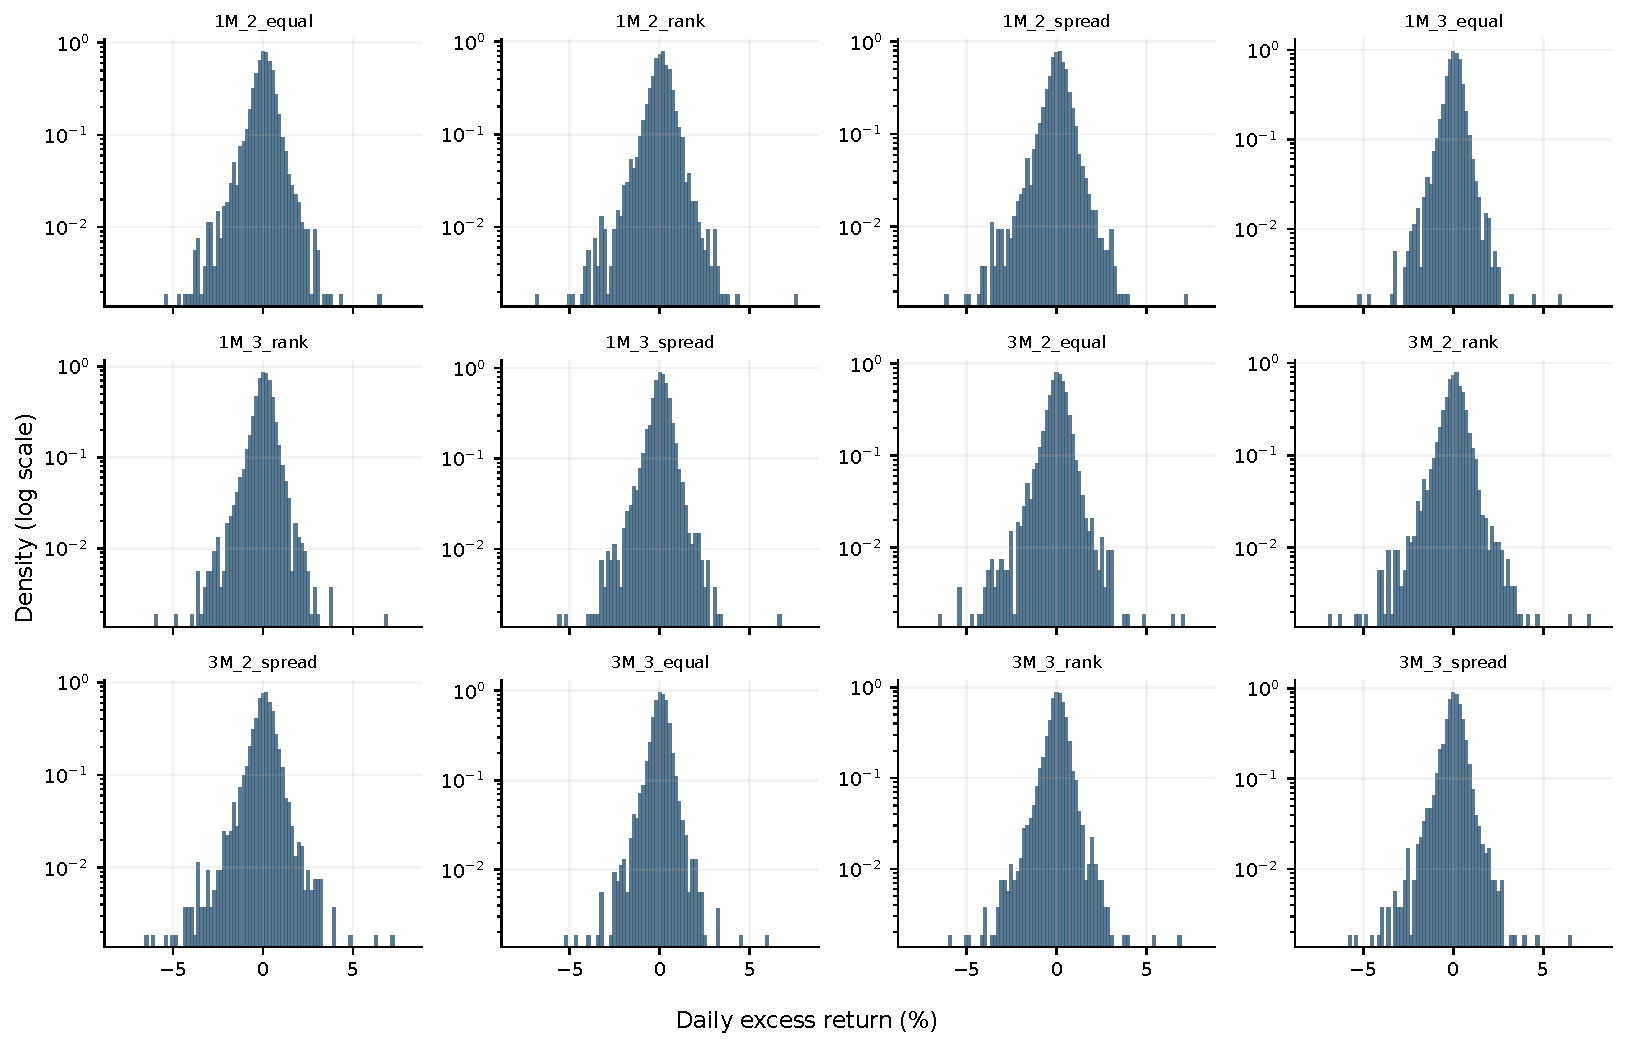
\includegraphics[width=\linewidth,height=6.2in,keepaspectratio]{../results/figures/baseline_distributions.pdf}\caption{\textbf{All twelve baseline return distributions.} Daily arithmetic excess-return histograms with log density. Shared plotted bins emphasize differences across portfolios; reported moments and tail statistics use every observation, including any extreme outside these bins.}\label{appfig:baseline_distributions}\end{figure}
\clearpage
\begin{figure}[H]\centering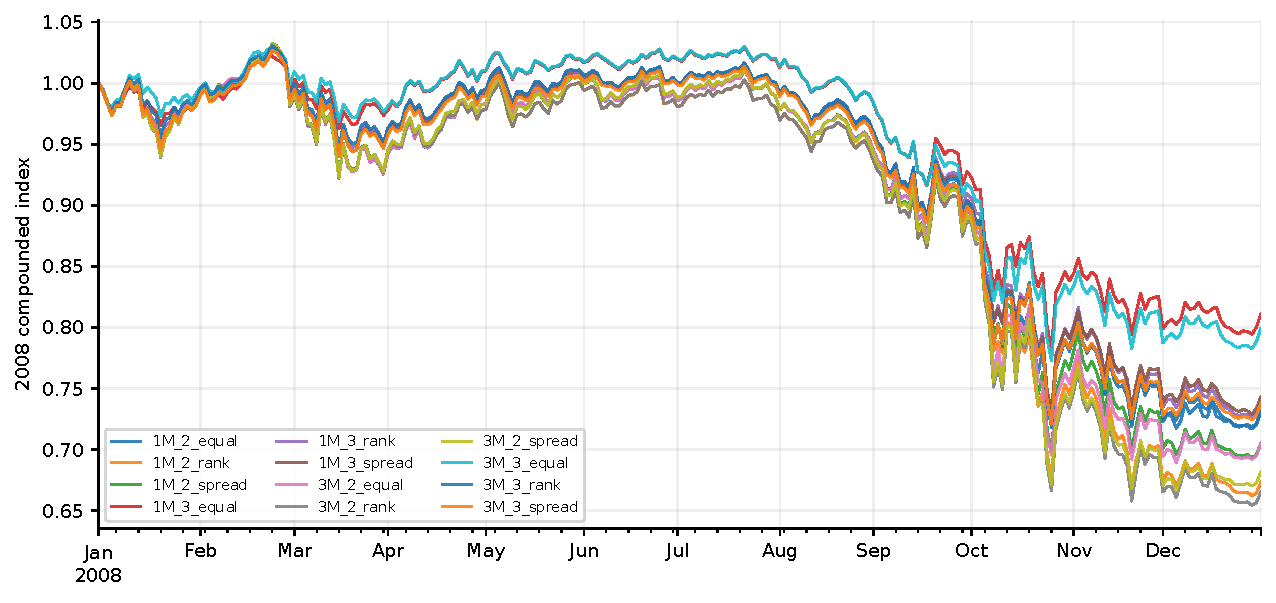
\includegraphics[width=\linewidth,height=6.2in,keepaspectratio]{../results/figures/baseline_2008.pdf}\caption{\textbf{Baseline portfolios during 2008.} Calendar-2008 compounded excess-return indices for all twelve constructions, rebased at the start of the episode. Crisis returns remain included in the full-sample comparisons.}\label{appfig:baseline_2008}\end{figure}
\clearpage
\begin{figure}[H]\centering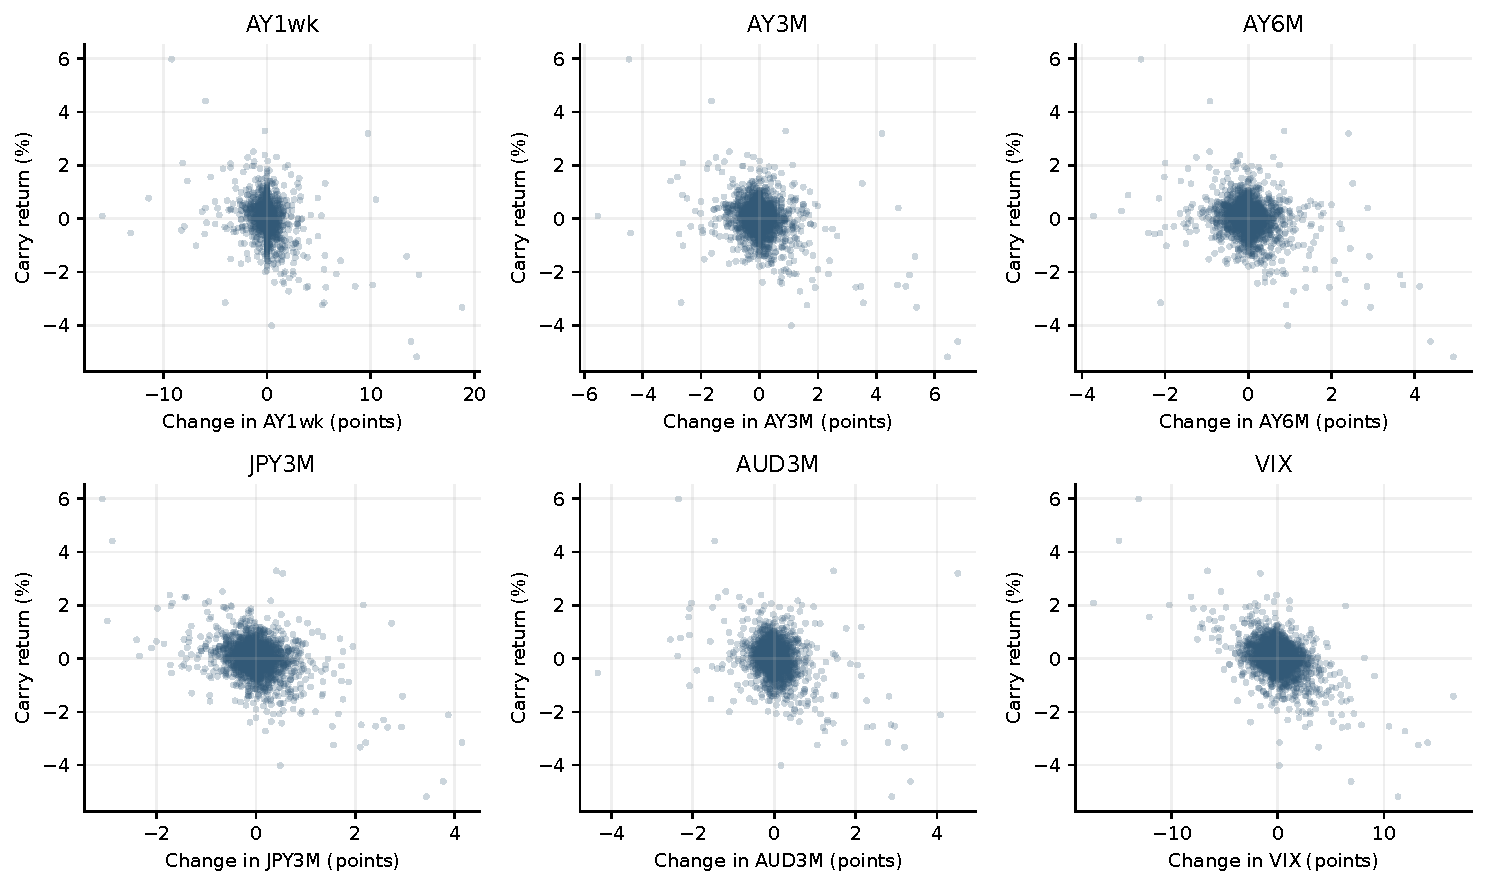
\includegraphics[width=\linewidth,height=6.2in,keepaspectratio]{../results/figures/volatility_scatter.pdf}\caption{\textbf{Carry and contemporaneous volatility changes.} Baseline daily carry returns versus same-period changes in all six volatility indicators. This describes contemporaneous co-movement, rather than a forecast available before the return.}\label{appfig:volatility_scatter}\end{figure}
\clearpage
\begin{figure}[H]\centering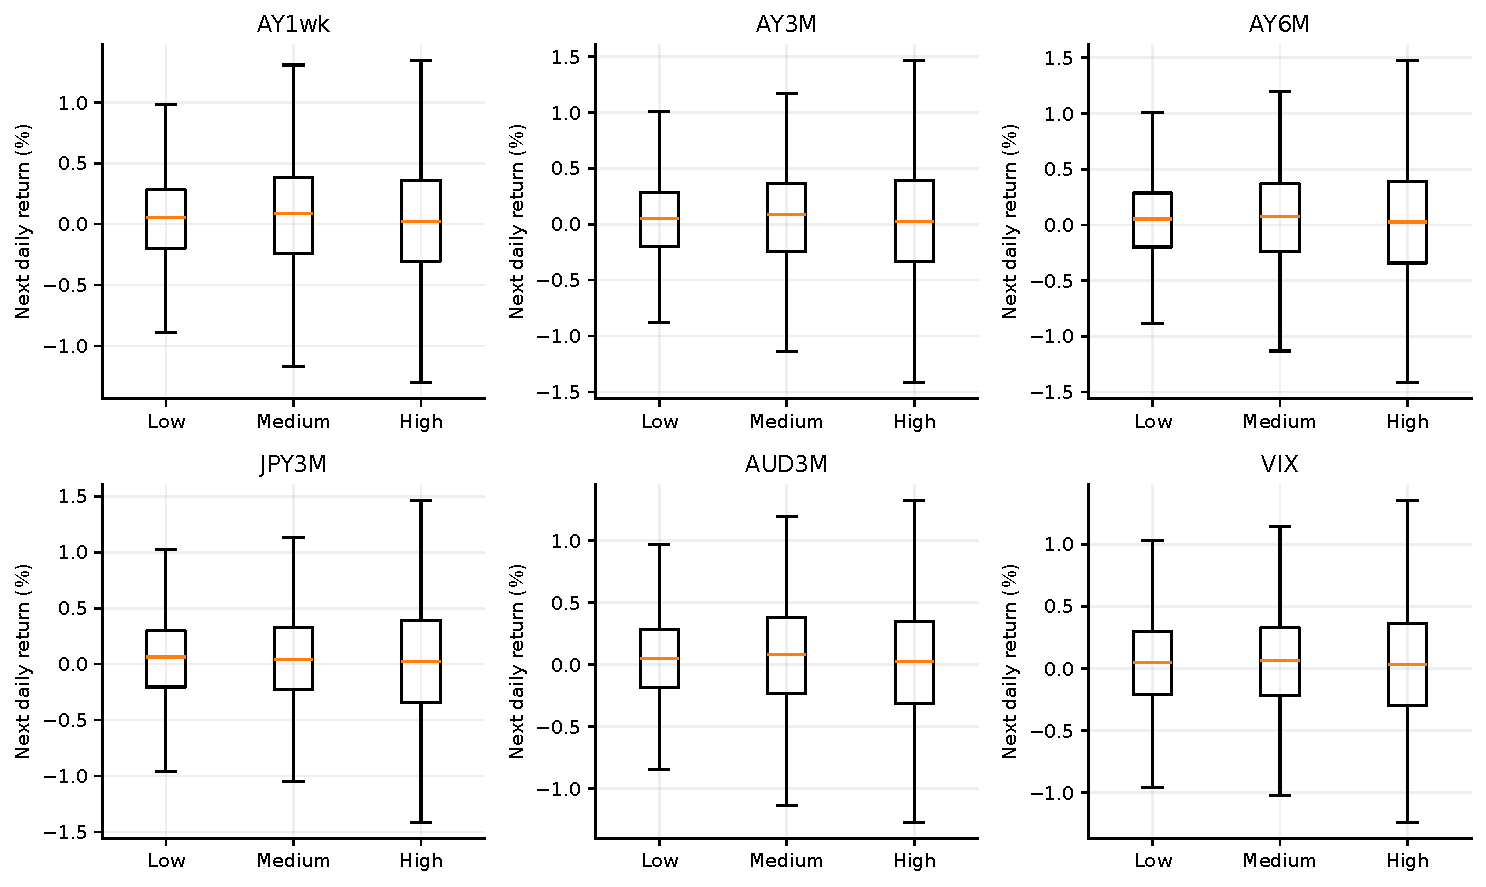
\includegraphics[width=\linewidth,height=6.2in,keepaspectratio]{../results/figures/predictive_regime_distributions.pdf}\caption{\textbf{Subsequent returns by observed volatility regime.} Next-period baseline carry returns grouped by previously observed low, medium and high volatility regimes for each indicator. Outlier markers are suppressed for legibility; tail observations remain in the regime statistics.}\label{appfig:predictive_regime_distributions}\end{figure}
\clearpage
\begin{figure}[H]\centering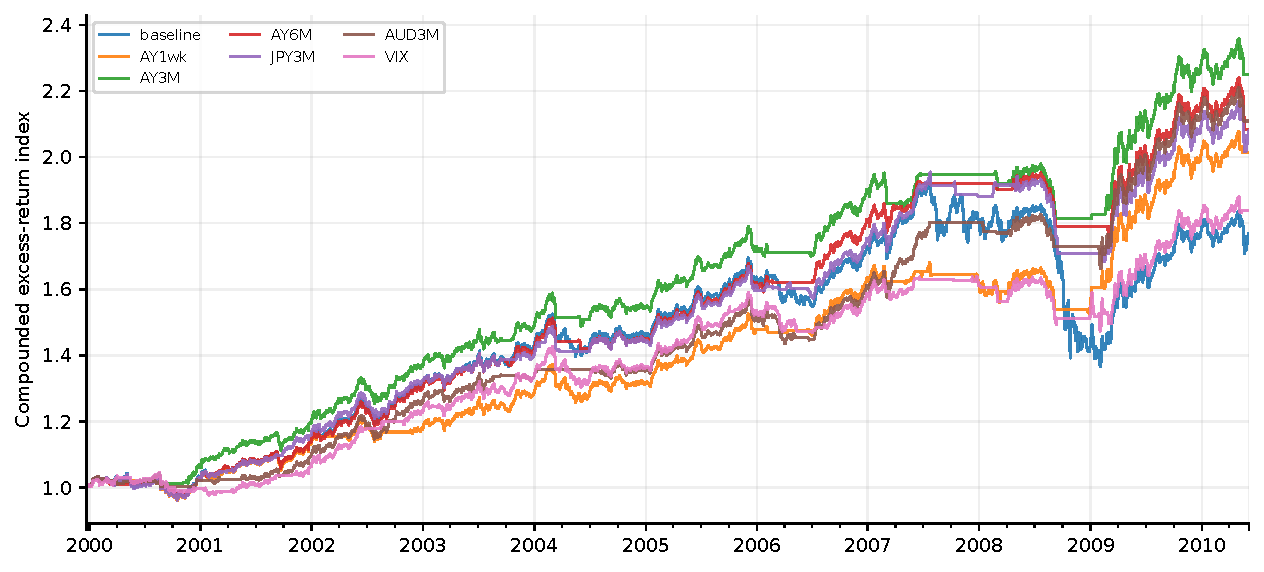
\includegraphics[width=\linewidth,height=6.2in,keepaspectratio]{../results/figures/conditioned_wealth.pdf}\caption{\textbf{All six volatility-conditioned wealth paths.} The baseline and all six fixed-rule filters share the 2,727-date eligible sample. Thresholds use the preceding 252 observations and exposure decisions apply to subsequent returns; inactive FX positions earn zero excess return.}\label{appfig:conditioned_wealth}\end{figure}
\clearpage
\begin{figure}[H]\centering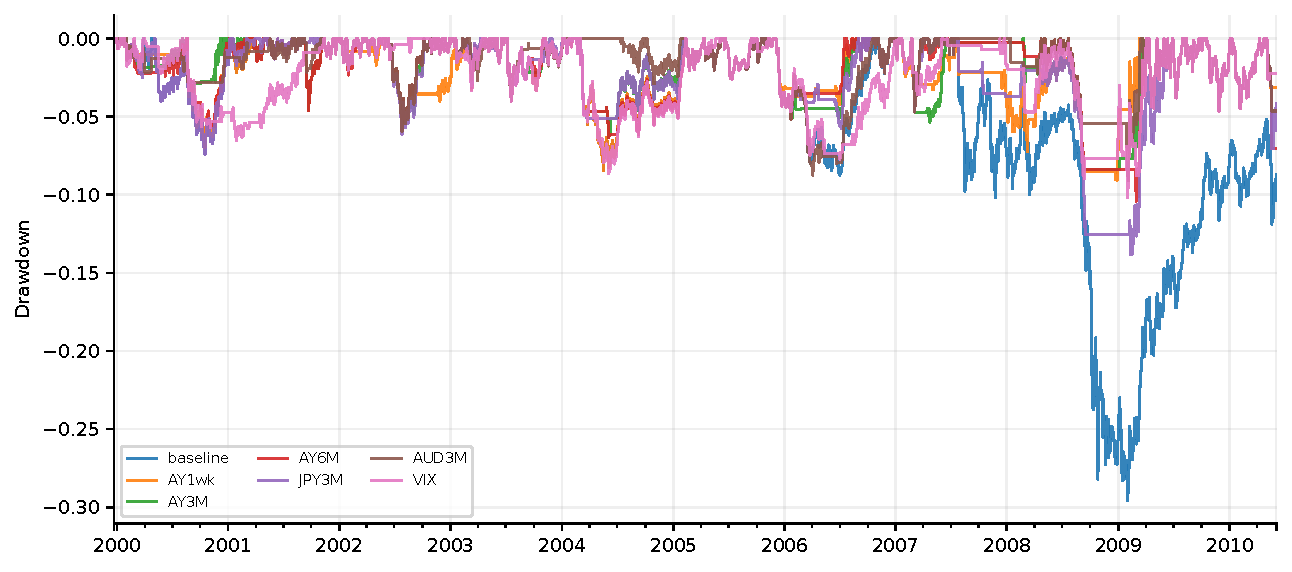
\includegraphics[width=\linewidth,height=6.2in,keepaspectratio]{../results/figures/conditioned_drawdowns.pdf}\caption{\textbf{All six volatility-conditioned drawdown paths.} Drawdowns on the same six-filter comparison sample. Reduced market exposure contributes to protection; the main text separately compares exposure-matched and volatility-matched controls.}\label{appfig:conditioned_drawdowns}\end{figure}
\clearpage
\begin{figure}[H]\centering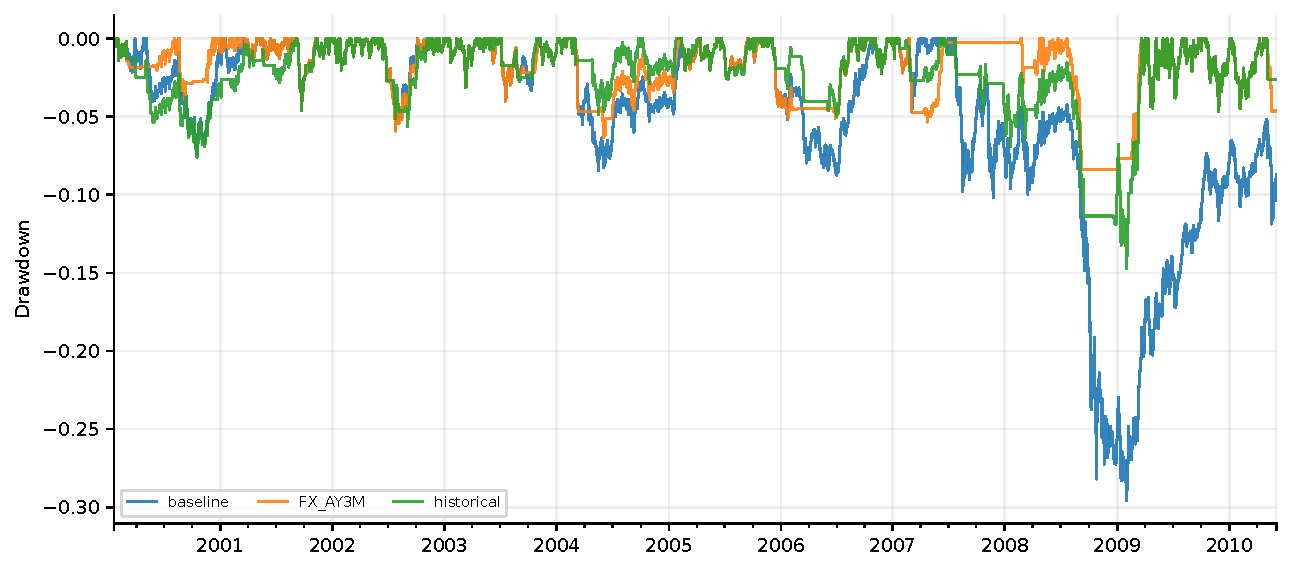
\includegraphics[width=\linewidth,height=6.2in,keepaspectratio]{../results/figures/historical_drawdowns.pdf}\caption{\textbf{Historical versus implied conditioning: drawdowns.} The baseline, AY3M-implied filter and 21-day AUD/JPY realized-volatility filter use identical 2,707 evaluation dates. The main text provides the corresponding wealth and distribution figures and uncertainty comparison.}\label{appfig:historical_drawdowns}\end{figure}
\end{document}
